\documentclass[a4paper,12pt]{ctexart}
%\usepackage[utf8]{inputenc} % ctexart 已经处理了编码,通常不需要这两个包
%\usepackage[T1]{fontenc}
\usepackage{amsmath}
\usepackage{graphicx}
\usepackage{geometry}
\usepackage{circuitikz} % 用于绘制电路图
\usepackage{float}
\usepackage{hyperref}

\geometry{left=2.5cm,right=2.5cm,top=2.5cm,bottom=2.5cm}

\title{基于模拟电路的PID控制器设计与分析}
\author{孙智诚 \\ 模拟电路课程设计}
\date{\today}

\begin{document}

\maketitle

\begin{abstract}
过往的学习和实践中,笔者往往通过算法来实现PID控制器,本文意欲以模拟电路的形式,构建一种响应更精确、更迅速,成本更低的PID控制器,因其结构简单、不用编程,
故可以在一些较为基础的场景进行应用,同时也能用以让笔者更加深刻地了解放大电路中积分器、微分器的实际意义。
\end{abstract}



\section{PID控制理论}

PID控制器的输出 $u(t)$ 与输入误差 $e(t)$ 的关系为:
\begin{equation}
    u(t) = K_p e(t) + K_i \int_{0}^{t} e(\tau) d\tau + K_d \frac{de(t)}{dt}
\end{equation}
其中,$K_p$ 为比例系数,$K_i$ 为积分系数,$K_d$ 为微分系数。也就是说,控制器拿到误差 $e(t)$ 后,并不是只关注当前的误差状态,而是把误差拆成三种不同角度的量来处理,然后把三部分结果叠加成最终的控制输出 $u(t)$。

\subsection{误差与闭环的基本逻辑}
在闭环控制中,误差一般定义为
\begin{equation}
    e(t) = r(t) - y(t)
\end{equation}
其中 $r(t)$ 为期望输入,$y(t)$ 为实际反馈值。PID的目的并不复杂:通过合理设计 $u(t)$ 的大小与方向,让系统输出 $y(t)$ 尽可能贴近 $r(t)$。

\subsection{比例项 \texorpdfstring{\(P\)}{P}}
比例项为 $u_P(t) = K_p e(t)$。它的意义很直观:误差越大,纠正力度越大。
因此 $K_p$ 往往是调参时首先关注的变量。
当 $K_p$ 较小时,系统响应偏慢,输出跟随设定值不够积极,可能出现较明显的稳态误差;
当 $K_p$ 逐渐增大时,响应会更快,但过大时容易带来超调甚至振荡。

在实际电路中,比例项对应的就是一个线性放大环节;如果后续环节本身存在饱和或限幅,那么单纯增大 $K_p$ 往往并不能无限提高效果,反而可能把系统推向不稳定。

\subsection{积分项 \texorpdfstring{\(I\)}{I}}
积分项为
$
    u_I(t) = K_i \int_{0}^{t} e(\tau) d\tau
$,
它的核心作用是消除稳态误差,只要误差长期不为零,积分就会不断累加,直到把误差推回到接近零的范围。
但积分也有明显的副作用:当系统存在输出限幅、执行器能力不足或起始误差过大时,积分项可能在短时间内累积过多,造成较大的超调;这种现象在控制中常被称为积分windup或者超调。
因此,在模拟电路实现时通常会配合一定的限幅措施,例如在积分电容并联大电阻,或在输出端加钳位,以避免积分项无限累积。

\subsection{微分项 \texorpdfstring{\(D\)}{D}}
微分项为
$u_D(t) = K_d \frac{de(t)}{dt}$,
它反映的是误差变化的快慢。当误差变化很快时,微分项会给出一个减缓其变化速率的纠正量,从而改善系统的动态过程,例如降低超调、加快收敛。
然而,微分对高频噪声非常敏感:噪声往往表现为快速抖动,经过微分后会被放大,导致控制输出抖动甚至引起电路自激。
因此工程上常用“带限微分”,即在微分网络中加入电阻或电容,形成高频滚降,而不是理想微分。

\subsection{本设计采用PID的动机}
综合来看,$P$ 负责提供基本控制力度,$I$ 用于消除稳态误差,$D$ 则在动态过程中起到抑制超调与改善响应的作用。本文后续将围绕模拟电路实现的可行性,分别给出比例、积分、微分环节的电路结构与参数设计方法,并通过仿真验证其在典型输入(如阶跃)下的响应特性。


\section{模拟电路设计}
本节将基于前文的控制理论基础,在本学期模拟电路课程学习的知识的基础上寻找对应的
解决方案,设计符合PID控制器基本原理的模拟电路,并在此基础上尝试进行优化,以满足
实际的使用需求。
\subsection{比例环节 \texorpdfstring{\(P\)}{P}}
比例环节用运放反相放大器实现,其传递函数可写为
\begin{equation}
    G_P(s) = -\frac{R_f}{R_{in}}
\end{equation}
因此比例系数的等效关系为 $K_p = \frac{R_f}{R_{in}}$。
在实际搭建时,我们可以使用电位器作为 $R_f$ 或 $R_{in}$ 的一部分,以便于在实验中对 $K_p$ 做连续调节,找到我们
需要的比例系数。

\begin{figure}[H]
    \centering
    \begin{circuitikz}[american]
        % Define op-amp position
        \draw (3,0) node[op amp] (opamp) {};
        
        % Input signal and input resistor to inverting input (-)
        \draw (opamp.-) -- ++(-1,0) coordinate(invnode)
              to[R,l=$R_{in}$] ++(-2,0) 
              to[short,-o] ++(-0.5,0) node[left]{$V_{in}$};
        
        % Non-inverting input (+) directly to ground
        \draw (opamp.+) -- ++(0,-0.8) node[ground]{};
        
        % Output
        \draw (opamp.out) -- ++(1.5,0) coordinate(outnode) 
              to[short,-o] ++(0.5,0) node[right]{$V_{out}$};
        
        % Feedback resistor from output to inverting input
        \draw (outnode) |- ++(0,1.5) coordinate(fbnode)
              to[R,l=$R_f$] (fbnode -| invnode) |- (invnode);
        
       
    \end{circuitikz}
    \caption{比例环节 运放反相放大器}
\end{figure}

\subsection{积分环节 \texorpdfstring{\(I\)}{I}}
积分环节采用经典运放积分器:输入端为电阻 $R$,反馈为电容 $C$。理想情况下的传递函数为
\begin{equation}
    G_(s) = -\frac{1}{RCs}
\end{equation}
对应到PID中的参数关系为 $K_i = \frac{1}{RC}$。
需要指出的是,理想积分器对直流增益无穷大,实际电路中会因运放失调、
偏置电流等导致输出缓慢漂移并最终饱和。因此工程上通常在反馈电容两端并联一个较大的电阻 $R_b$,形成带泄放的积分器,使低频增益有限,从而提升长期稳定性。

\begin{figure}[H]
    \centering
    \begin{circuitikz}[american]
        % Define op-amp position
        \draw (3,0) node[op amp] (opamp) {};
        
        % Input signal and input resistor to inverting input (-)
        \draw (opamp.-) -- ++(-1,0) coordinate(invnode)
              to[R,l=$R$] ++(-2,0) 
              to[short,-o] ++(-0.5,0) node[left]{$V_{in}$};
        
        % Non-inverting input (+) directly to ground
        \draw (opamp.+) -- ++(0,-0.8) node[ground]{};
        
        % Output
        \draw (opamp.out) -- ++(1.5,0) coordinate(outnode) 
              to[short,-o] ++(0.5,0) node[right]{$V_{out}$};
        
        % Feedback capacitor (with parallel resistor) from output to inverting input
        \draw (outnode) |- ++(0,1.75) coordinate(fbnode);
        
        % Capacitor C in feedback (top path)
        \draw (fbnode) to[C,l=$C$] (fbnode -| invnode) coordinate(fbend) |- (invnode);
        

        \end{circuitikz}
    \caption{积分环节 运放积分器(反馈电容 $C$ 或许还可以并联一个泄放电阻 $R_b$)}
\end{figure}
由于本电路较为基础,故而笔者并未选择进行软件仿真,而是在学校实验室,利用现有的op-amp
与元器件进行了试验。电路中选用了$R=500k\Omega \quad C=0.2\mu F$,使得时间常数$\tau=0.5s$,
为了便于观察,笔者在$V_{out}$后追加了一个$\frac{R_{f}}{R_{in}}=1$的反相op-amp,
以此将第一级放大电路反转的信号复原为原本的相位。通过输入方波信号,得到以下$v_i-t$与$v_o-t$特性曲线:
\begin{figure}[H]
    \centering
    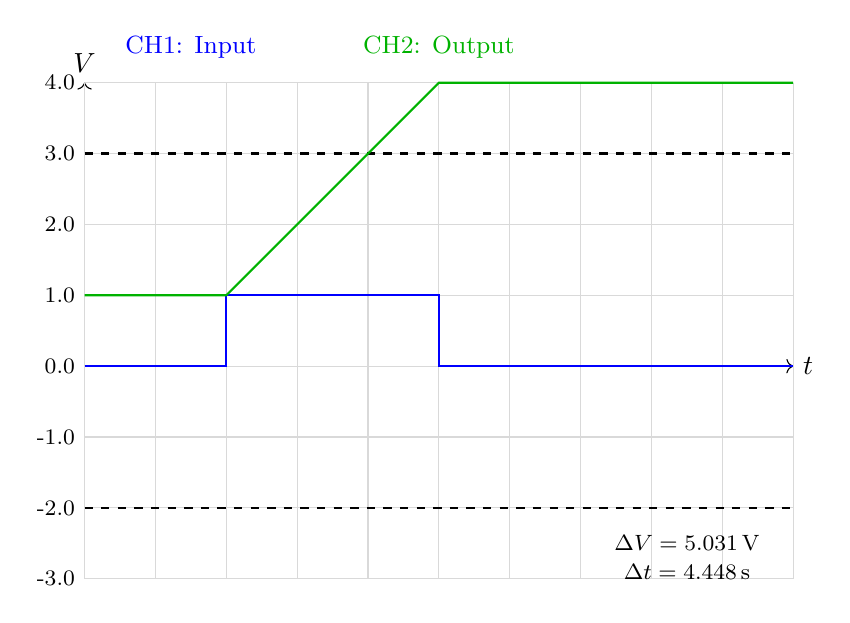
\begin{tikzpicture}[scale=0.9]
        % Draw axes
        \draw[->] (0,0) -- (10,0) node[right] {$t$};
        \draw[->] (0,-3) -- (0,4) node[above] {$V$};
        
        % Grid (light gray)
        \foreach \x in {0,1,...,10} {
            \draw[gray!30] (\x,-3) -- (\x,4);
        }
        \foreach \y in {-3,-2,-1,0,1,2,3,4} {
            \draw[gray!30] (0,\y) -- (10,\y);
        }
        
        % Y-axis labels
        \foreach \y in {-3,-2,-1,0,1,2,3,4} {
            \node[left,font=\footnotesize] at (0,\y) {\y.0};
        }
        
        % Horizontal reference lines (dashed)
        \draw[dashed,thick] (0,3) -- (10,3);
        \draw[dashed,thick] (0,-2) -- (10,-2);
        
        % Input square wave (blue, CH6 style)
        \draw[blue,thick] (0,0) -- (2,0) -- (2,1) -- (5,1) -- (5,0) -- (10,0);
        
        % Output integrated ramp (green, CH2 style)
        % When input is 1V (from t=2 to t=5), output ramps up with slope 1/RC = 1/0.5 = 2
        % From V=1 at t=2, slope=2, so at t=5 (delta_t=3), V_out = 1 + 2*3 = 7 (but clamp to 4)
        \draw[green!70!black,thick] 
            (0,1) -- (2,1)  % constant at 1V
            -- (5,4)        % ramp up (slope=2)
            -- (10,4);      % hold at saturation
        
        % Channel labels (top)
        \node[blue,above] at (1.5,4.2) {\small CH1: Input};
        \node[green!70!black,above] at (5,4.2) {\small CH2: Output};
        
        % Time and voltage delta annotation (bottom right, like in the reference)
        \node[align=left,font=\footnotesize] at (8.5,-2.5) {$\Delta V = 5.031\,\text{V}$};
        \node[align=left,font=\footnotesize] at (8.5,-2.9) {$\Delta t = 4.448\,\text{s}$};
        
    \end{tikzpicture}
    \caption{时间常数 $\tau=0.5$ 时的响应曲线}
\end{figure}
\subsubsection{PI控制器}
更进一步地,我们可以结合前面提及的比例放大器,设计出比例-积分放大器,
也就是工程中常用的PI控制器。通过添加一个输出限幅部分,
它可以满足大多数的控制需求,同时也可以比较粗糙地避免过调发生。

PI控制器的传递函数可以写为:
\begin{equation}
    G_{PI}(s) = K_p + \frac{K_i}{s} = K_p\left(1 + \frac{1}{T_i s}\right)
\end{equation}
其中 $T_i = K_p/K_i$ ,为积分时间常数。在运放实现中,可以采用单运放结构:在反馈网络中将电阻和电容串联,输入端仍为电阻。此时反馈阻抗为 $Z_f = R_f + \frac{1}{sC_f}$,传递函数为:
\begin{equation}
    G_{PI}(s) = -\frac{R_f + \frac{1}{sC_f}}{R_{in}} = -\frac{R_f}{R_{in}}\left(1 + \frac{1}{sR_fC_f}\right)
\end{equation}
比较可得:$K_p = \frac{R_f}{R_{in}}$,$T_i = R_fC_f$。

为了防止积分饱和和输出超过执行器或后级电路的耐受范围,在输出端加入限幅电路。常用的限幅方案包括:
\begin{itemize}
    \item \textbf{二极管钳位}:使用稳压二极管或普通二极管配合基准电压,将输出钳制在指定范围内。
    \item \textbf{运放饱和保护}:利用运放本身的电源轨限制输出范围,如 $\pm 12V$ 供电时输出约为 $\pm 10V$。
\end{itemize}

\begin{figure}[H]
    \centering
    \begin{circuitikz}[american, scale=1.0]
        % Define op-amp position
        \draw (3,0) node[op amp] (opamp) {};
        
        % Input signal and input resistor to inverting input (-)
        \draw (opamp.-) -- ++(-1,0) coordinate(invnode)
              to[R,l=$R_{in}$] ++(-2,0) 
              to[short,-o] ++(-0.5,0) node[left]{$V_{in}$};
        
        % Non-inverting input (+) directly to ground
        \draw (opamp.+) -- ++(0,-0.8) node[ground]{};
        
        % Output 
        \draw (opamp.out) -- ++(1.5,0) coordinate(outnode);
        
        % Feedback network: Cf (capacitor first) then Rf (resistor second), in series
        \draw (outnode) |- ++(0,1.5) coordinate(fbtop);
        
        % Capacitor Cf first (closer to output)
        \draw (fbtop) to[C,l=$C_f$] ++(-2,0) coordinate(fbmid);
        
        % Resistor Rf second (closer to inverting input)
        \draw (fbmid) to[R,l_=$R_f$] (fbmid -| invnode) |- (invnode);
        
        % Limiting circuit: two Zener diodes to ground (anti-parallel)
       
        \draw (outnode) -- ++(0.7,0) coordinate(dlimit)
            (dlimit) to[zzDo,l_=$D_1$] ++(0,1.5) node[above]{$+V_{lim}$};
        \draw (dlimit) to[zzDo,l_=$D_2$,invert] ++(0,-1.5) node[below]{$-V_{lim}$};
        % Final output terminal
        \draw (outnode) -- ++(1,0) to[short,-o] ++(0.5,0) node[right]{$V_{out}$};
        
    \end{circuitikz}
    \caption{PI控制器(反馈为 $C_f$ 与 $R_f$ 串联,输出端稳压二极管限幅)}
\end{figure}

这类控制器也是笔者在实际控制中运用最多的控制器。相较完整的PID控制器,它的调参更为简单,且通过直接限幅,可以将输出严格限定在要求范围内。为了验证PI控制器的实际效果,笔者搭建了参数为 $K_p=1.0$、$T_i=0.5$ 的PI控制器,并输入周期性方波信号进行测试。图中展示了输入信号、比例输出、积分输出以及经限幅后的总输出波形:

\begin{figure}[H]
    \centering
    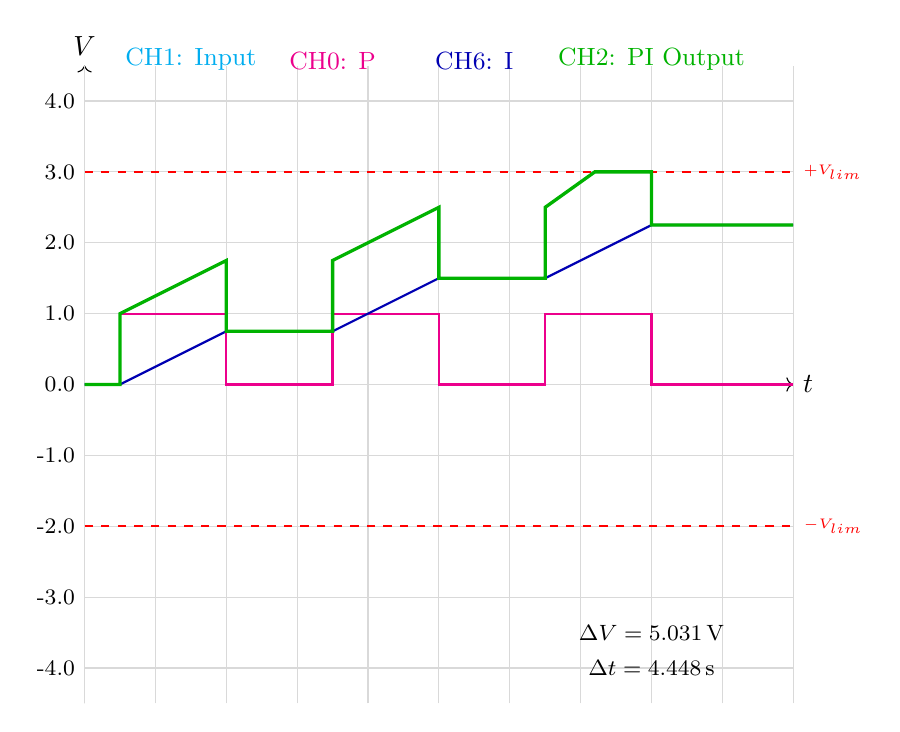
\begin{tikzpicture}[scale=0.9]
        % Draw axes
        \draw[->] (0,0) -- (10,0) node[right] {$t$};
        \draw[->] (0,-4.5) -- (0,4.5) node[above] {$V$};
        
        % Grid (light gray)
        \foreach \x in {0,1,...,10} {
            \draw[gray!30] (\x,-4.5) -- (\x,4.5);
        }
        \foreach \y in {-4,-3,-2,-1,0,1,2,3,4} {
            \draw[gray!30] (0,\y) -- (10,\y);
        }
        
        % Y-axis labels
        \foreach \y in {-4,-3,-2,-1,0,1,2,3,4} {
            \node[left,font=\footnotesize] at (0,\y) {\y.0};
        }
        
        % Horizontal reference lines for limits (dashed red)
        \draw[dashed,red,thick] (0,3) -- (10,3) node[right,font=\tiny] {$+V_{lim}$};
        \draw[dashed,red,thick] (0,-2) -- (10,-2) node[right,font=\tiny] {$-V_{lim}$};
        
        % Input square wave (cyan/blue, CH1) - periodic
        \draw[cyan,thick] (0,0) -- (0.5,0) -- (0.5,1) -- (2,1) -- (2,0) -- (3.5,0) -- (3.5,1) -- (5,1) -- (5,0) -- (6.5,0) -- (6.5,1) -- (8,1) -- (8,0) -- (10,0);
        
        % Proportional output (purple/magenta, CH0) - follows input instantly
        \draw[magenta,thick] (0,0) -- (0.5,0) -- (0.5,1) -- (2,1) -- (2,0) -- (3.5,0) -- (3.5,1) -- (5,1) -- (5,0) -- (6.5,0) -- (6.5,1) -- (8,1) -- (8,0) -- (10,0);
        
        % Integral output (blue, CH6) - ramp during high, constant during low
        \draw[blue!70!black,thick] 
            (0,0) -- (0.5,0)      % low period
            -- (2,0.75)           % ramp up during high
            -- (3.5,0.75)         % hold during low
            -- (5,1.5)            % ramp up during high
            -- (6.5,1.5)          % hold during low
            -- (8,2.25)           % ramp up during high
            -- (10,2.25);         % hold during low
        
        % PI output with limiting (green, CH2)
        % PI = P + I, but clamped at ±Vlim
        \draw[green!70!black,very thick] 
            (0,0) -- (0.5,0)      % initial zero
            -- (0.5,1)            % jump (P component)
            -- (2,1.75)           % ramp up (P+I)
            -- (2,0.75)           % drop when input goes low (only I remains)
            -- (3.5,0.75)         % hold
            -- (3.5,1.75)         % jump (P component)
            -- (5,2.5)            % ramp up
            -- (5,1.5)            % drop
            -- (6.5,1.5)          % hold
            -- (6.5,2.5)          % jump
            -- (7.2,3)            % ramp up to limit
            -- (8,3)              % clamped at +Vlim
            -- (8,2.25)           % drop when input goes low
            -- (10,2.25);         % hold
        
        % Channel labels (top)
        \node[cyan,above] at (1.5,4.3) {\small CH1: Input};
        \node[magenta,above] at (3.5,4.3) {\small CH0: P};
        \node[blue!70!black,above] at (5.5,4.3) {\small CH6: I};
        \node[green!70!black,above] at (8.0,4.3) {\small CH2: PI Output};
        
        % Annotation (bottom right)
        \node[align=left,font=\footnotesize] at (8,-3.5) {$\Delta V = 5.031\,\text{V}$};
        \node[align=left,font=\footnotesize] at (8,-4.0) {$\Delta t = 4.448\,\text{s}$};
        
    \end{tikzpicture}
    \caption{PI控制器响应曲线,$K_p=1.0$,$T_i=0.5$,输入周期性方波,输出限幅于 $\pm V_{lim}$}
\end{figure}

从波形中可以清晰地看到PI控制器的工作特性:输入方波(青色CH1)经过比例环节(紫色CH0)得到即时响应,积分环节(蓝色CH6)则在每个高电平期间累积上升,低电平期间保持不变。两者叠加形成的PI输出(绿色CH2)在第一、二周期正常工作,但在第三周期因积分持续累积而触发稳压二极管限幅,被钳制在 $+V_{lim}$ 附近,有效避免了输出过冲对后级电路的损害。当输入回到低电平时,输出立即下降(失去比例分量),仅保留积分值。这种限幅特性正是实际工程应用中保护执行器的重要手段,同时也揭示了PI控制器在持续偏差输入下的积分饱和现象。

\subsection{微分环节 \texorpdfstring{\(D\)}{D} (Derivative Stage)}
微分环节的理想形式为 $G_D(s)=K_d s$,但理想微分会显著放大高频噪声。为避免输出抖动与自激,本设计采用带限微分(超前环节)的实现方式:输入串联 $C_d$ 与 $R_d$ 形成高通特性,反馈端再通过小电容/电阻形成高频滚降,使得微分只在目标频段内发挥作用。
在参数设计上,微分通道更关注有效频带与噪声抑制,而不是盲目追求“微分越强越好”。

\subsection{求和与输出整形 (Summing and Output Shaping)}
将 $P$、$I$、$D$ 三路输出用运放反相加法器进行求和,得到控制输出 $u(t)$。反相加法器的一个优点是各路权重可以直接用输入电阻比值体现,便于参数标定与调整。
此外,考虑到实际执行机构(电机驱动、功率级等)通常存在输入范围限制,输出端可加入对称限幅(如二极管钳位或运放供电限幅下的饱和保护),以减少因过大控制量导致的积分饱和现象。

\section{参数计算与仿真 (Simulation and Results)}
\subsection{参数选择}
列出选用的电阻、电容值,以及对应的 $K_p, K_i, K_d$ 计算值。

\subsection{仿真波形}
展示输入阶跃信号时,P、I、D各环节的输出波形,以及总输出波形。

\section{结论 (Conclusion)}
总结设计的优缺点,以及未来改进方向。

\begin{thebibliography}{99}
\bibitem{ref1} 模拟电子技术基础教材.
\bibitem{ref2} 相关电路设计手册.
\end{thebibliography}

\end{document}
